Рассмотрим задачу определения новых положений узлов расчетной сетки немного в другой постановке.
Пусть для каждого узла $\vec{N}$ известна линейная скорость нарастания льда $v(\vec{N})$ (в метрах в секунду).
Будем считать, что нарастание льда в любой точке роста выполняется одновременно во всех направлениях аналогично принципу Гюйгенса-Френеля распространения волн.
Тогда фронт распространения льда от произвольной точки $\vec{P}$ через промежуток времени $\Delta t$ будет иметь форму сферы с центром в точке $\vec{P}$ и радиусом $v(\vec{P}) \Delta t$.
Далее будем предполагать, что выполняется расчет новых положений узлов через некоторый фиксированный момент времени $\Delta t$, то есть для каждого узла известен радиус продвижения фронта льда $R(\vec{N}) = v(\vec{N}) \Delta t$.
Так как элементами расчетной сетки являются треугольники, то необходимо определить радиус продвижения фронта льда для каждой внутренней точки треугольника по данным его вершин.

Рассмотрим ячейку расчетной сетки, вершинами которой являются точки $\vec{A}$, $\vec{B}$, $\vec{C}$.
Точки треугольника представляют собой геометрическое место точек, описываемое следующим образом:

\begin{equation}
\begin{cases}
\vec{P}(\beta, \gamma) = \vec{A} + \beta (\vec{B} - \vec{A}) + \gamma (\vec{C} - \vec{A}) = \vec{A} + \beta \vec{AB} + \gamma \vec{AC} \\
\beta \ge 0 \\
\gamma \ge 0 \\
\beta + \gamma \le 1
\end{cases}
\end{equation}

Определим для каждой точки треугольника $\vec{P}(\beta, \gamma)$ радиус продвижения фронта льда как $R(\vec{P}(\beta, \gamma)) = R(\beta, \gamma) = R(\vec{A}) + \beta (R(\vec{B}) - R(\vec{A})) + \gamma (R(\vec{C}) - R(\vec{A})) = R_A + \beta R_{AB} + \gamma R_{AC}$.
Фронт продвижения льда от точки $\vec{P}(\beta, \gamma)$ представляет собой сферу $S(\beta, \gamma) = S(\vec{P}(\beta, \gamma), R(\beta, \gamma))$.
Фронтом продвижения льда всей треугольной ячейки будем считать общую огибающую сфер, построенных на всех точках этой ячейки, что показано на Fig.~\ref{fig:pic_general_envelope_size}.

\begin{figure}
  \centering
  \begin{minipage}[b]{0.48\textwidth}
    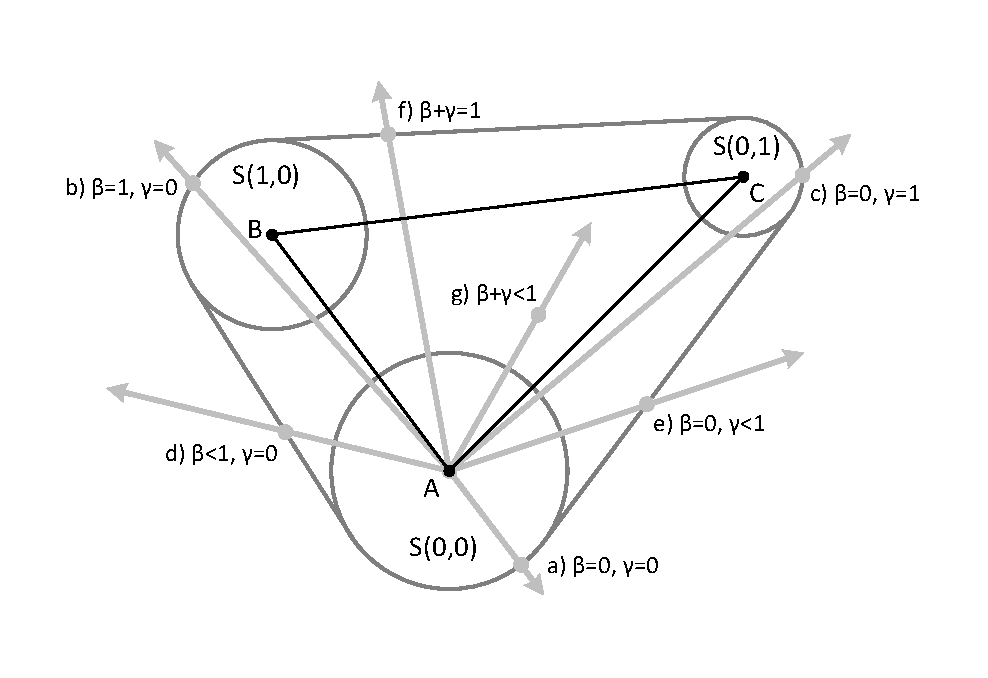
\includegraphics[width=\textwidth]{pics/pic_general_envelope_size.pdf}
    \caption{Общая огибающая поверхность сфер, построенных на точках треугольника.}\label{fig:pic_general_envelope_size}
  \end{minipage}
  \hfill
  \begin{minipage}[b]{0.48\textwidth}
    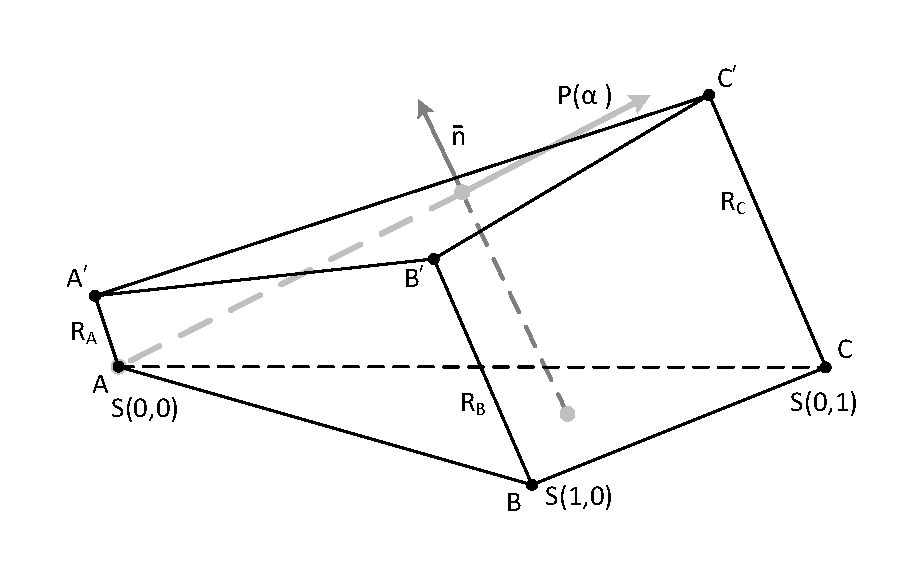
\includegraphics[width=\textwidth]{pics/pic_general_envelope_2_size.pdf}
    \caption{Поиск нового положения узла на общей касательной плосткости трех сфер.}\label{fig:pic_general_envelope_2_size}
  \end{minipage}
\end{figure}

При изменении положения узлов расчетной сетки (точки $\vec{A}$, $\vec{B}$, $\vec{C}$) будем исходить из предположения, что после перемещения узлы будут находиться на общей огибающей поверхности множества сфер $S(\beta, \gamma)$ (новые положения узлов -- точки $\vec{A'}$, $\vec{B'}$, $\vec{C'}$).
Пока в расчете не учитываем влияние соседних расчетных ячеек.
Без ограничения общности можно рассмотреть только одну вершину ячейки (точка $\vec{A}$).
Пусть траектория движения точки $\vec{A}$ описывается уравнением полупрямой $\vec{P}(\alpha) = \vec{A} + \alpha \vec{D}$ при $\alpha \ge 0$.
$\vec{D}$ -- вектор направления движения точки, можно считать, что $|\vec{D}| = 1$.
Для поиска точек пересечения траектории движения точки $\vec{P}(\alpha) = \vec{A} + \alpha \vec{D}$ с произвольной сферой $S(\beta, \gamma)$ необходимо подставить координаты точки $\vec{P}(\alpha)$ в уравнение сферы $|\vec{P} - \vec{C}(\beta, \gamma)| = R(\beta, \gamma)$, где $\vec{C}(\beta, \gamma)$ -- центр рассматриваемой сферы.
В результате получим следующее уравнение:

\begin{equation}\label{eqn:intersect}
|(\vec{A} + \alpha \vec{D}) - \vec{C}(\beta, \gamma)| = R(\beta, \gamma)
\end{equation}

Это уравнение нужно решить относительно неизвестной $\alpha$ при фиксированных параметрах $\beta$ и $\gamma$.
Это уравнение является квадратным, оно имеет не более двух корней, которые зависят от параметров $\alpha_{1,2} = \alpha_{1,2}(\beta, \gamma)$.
Для определения нового положения точки $\vec{A}$ необходимо найти максимальное значение вещественного корня такого уравнения для всех допустимых значений параметров.
При этом точка пересечения траектории движения точки $\vec{A}$ с общей огибающей семейства сфер может находиться на разных участках этой огибающей, что продемонстрировано на Fig.~\ref{fig:pic_general_envelope_size} и связано с условиями, которым удовлетворяют параметры $\beta$ и $\gamma$ (пункты a), b), c) -- пересечение со сферой с центром в вершинах треугольника, пункты d), e), f) -- пересечение со сферой с центром на ребрах треугольника, пункт g) -- пересечение со сферой с центром внутри треугольника).

Уравнение (\ref{eqn:intersect}) можно записать в виде $|\alpha \vec{D} - (\beta \vec{AB} + \gamma \vec{AC})|^2 = (R_A + \beta R_{AB} + \gamma R_{AC})^2$ или в явном виде как квадратное уравнение:

\begin{equation}
|\vec{D}|^2 \alpha^2 - 2(\beta (\vec{D}, \vec{AB}) + \gamma (\vec{D}, \vec{AC})) \alpha + |\beta \vec{AB} + \gamma \vec{AC}|^2 - (R_A + \beta R_{AB} + \gamma R_{AC})^2 = 0
\end{equation}

Наибольший корень этого уравнения (с учетом условия $|\vec{D}| = 1$) можно выписать в явном виде:

\begin{multline}
\alpha(\beta, \gamma) = \beta (\vec{D}, \vec{AB}) + \gamma (\vec{D}, \vec{AC}) + \\
\sqrt{(\beta (\vec{D}, \vec{AB}) + \gamma (\vec{D}, \vec{AC}))^2 - |\beta \vec{AB} + \gamma \vec{AC}|^2 + (R_A + \beta R_{AB} + \gamma R_{AC})^2}
\end{multline}

или

\begin{equation}
\begin{cases}
\alpha(\beta, \gamma) = k_{\beta} \beta + k_{\gamma} \gamma + \sqrt{T} \\
T = q_{\beta^2} \beta^2 + q_{\gamma^2} \gamma^2 + q_{\beta \gamma} \beta \gamma + q_{\beta} \beta + q_{\gamma} \gamma + q \\
k_{\beta} = (\vec{D}, \vec{AB}), k_{\gamma} = (\vec{D}, \vec{AC}) \\
q_{\beta^2} = (\vec{D}, \vec{AB})^2 - |\vec{AB}|^2 + R_{AB}^2, q_{\gamma^2} = (\vec{D}, \vec{AC})^2 - |\vec{AC}|^2 + R_{AC}^2 \\
q_{\beta \gamma} = 2 ((\vec{D}, \vec{AB})(\vec{D}, \vec{AC}) - (\vec{AB}, \vec{AC}) + R_{AB} R_{AC}) \\
q_{\beta} = 2 R_A R_{AB}, q_{\gamma} = 2 R_A R_{AC}, q = R_A^2
\end{cases}
\end{equation}

Для поиска нового положения точки $\vec{A}$ требуется найти максимум выражения $\alpha(\beta, \gamma)$ при условии соблюдения ограничений $\beta \ge 0$, $\gamma \ge 0$, $\beta + \gamma \le 1$.
Максимум выражения $\alpha(\beta, \gamma)$ достигается либо при условии нахождения центра сферы внутри треугольника, либо на одной из его сторон.

В случае нахождения центра сферы на стороне $AB$ треугольника $ABC$ выполняется условие $\gamma = 0$, и выражение для величины $\alpha$ имеет вид $\alpha_{\gamma = 0}(\beta) = k_{\beta} \beta + \sqrt{q_{\beta^2} \beta^2 + q_{\beta} \beta + q}$.
В случае нахождения центра сферы на стороне $AC$ треугольника $ABC$ выполняется условие $\beta = 0$, и выражение для величины $\alpha$ имеет вид $\alpha_{\beta = 0}(\gamma) = k_{\gamma} \gamma + \sqrt{q_{\gamma^2} \gamma^2 + q_{\gamma} \gamma + q}$.
В случае нахождения центра сферы на стороне $BC$ треугольника $ABC$ выполняется условие $\beta + \gamma = 1$, и выражение для величины $\alpha$ принимает следующий вид:

\begin{multline}
\alpha_{\beta + \gamma = 1}(\gamma) = (k_{\gamma} - k_{\beta}) \gamma + k_{\beta} + \\
\sqrt{(q_{\beta^2} + q_{\gamma^2} - q_{\beta \gamma}) \gamma^2 + (-2 q_{\beta^2} + q_{\beta \gamma} - q_{\beta} + q_{\gamma}) \gamma + (q_{\beta^2} + q_{\beta} + q)}
\end{multline}

Во всех случаях нахождения центра на одной из сторон треугольника задача нахождения максимального значения $\alpha(\beta, \gamma)$ при заданных ограничениях сводится к задаче поиска максимального значения функции вида $\alpha(x) = k_x x + k + \sqrt{q_{x^2} x^2 + q_x x + q}$ (с учетом этих ограничений), что не представляет труда (точкой максимума является либо точка локального экстремума, либо точка границы области определения функции).

Отдельно следует рассмотреть вариант, при котором центр искомой сферы находится внутри треугольника. В этом случае точка пересечения траектории $\vec{P}(\alpha) = \vec{A} + \alpha \vec{D}$ с общей огибающей находится на общей касательной плоскости к сферам $S(0, 0)$, $S(1, 0)$, $S(0, 1)$ (плоскость $A'B'C'$, см. Fig.~\ref{fig:pic_general_envelope_2_size}).

Центр искомой сферы находится с точке пересечения плоскости $ABC$ и прямой, проходящей через точку $\vec{P}(\alpha)$ и направленной вдоль нормали к плоскости $A'B'C'$.
Если вектор единичной нормали плоскости $A'B'C'$ обозначить через $\vec{n}$, то взаимосвязь точек плоскостей $ABC$ и $A'B'C'$ можно выразить следующим образом:

\begin{equation}
\begin{cases}
\vec{A'} = \vec{A} + \vec{n} R_A \\
\vec{B'} = \vec{B} + \vec{n} R_B \\
\vec{C'} = \vec{C} + \vec{n} R_C
\end{cases}
\end{equation}

Для нахождения вектора $\vec{n}$ воспользуемся тем фактом, что результат векторного произведения $\vec{A'B'} \times \vec{A'C'}$ коллинеарен вектору $\vec{n}$.
Запишем это в явном виде

\begin{equation}
(\vec{AB} + \vec{n} R_{AB}) \times (\vec{AC} + \vec{n} R_{AC}) = t \vec{n}
\end{equation}

\begin{equation}
\vec{AB} \times \vec{AC} + R_{AB} (\vec{n} \times \vec{AC}) - R_{AC} (\vec{n} \times \vec{AB}) = t \vec{n}
\end{equation}

\begin{equation}
t
\left[ { \begin{array}{c}
            n_x \\
            n_y \\
            n_z \\
         \end{array} } \right]
+ R_{AC}
\left[ { \begin{array}{c}
            n_y AB_z - n_z AB_y  \\
            n_z AB_x - n_x AB_z \\
            n_x AB_y - n_y AB_x \\
         \end{array} } \right]
- R_{AB}
\left[ { \begin{array}{c}
            n_y AC_z - n_z AC_y \\
            n_z AC_x - n_x AC_z \\
            n_x AC_y - n_y AC_x \\
         \end{array} } \right]
= \vec{AB} \times \vec{AC}
\end{equation}

Данное соотношение может выполняться при $t > 0$, либо при $t < 0$, что соответствует существованию двух общих касательных плоскостей к трем сферам.
Перепишем приведенное соотношение в виде системы линейных уравнений относительно составляющих нормали при произвольном значении параметра $t$.

\begin{equation}
\left[ { \begin{array}{ccc}
             t & R_{AC} AB_z - R_{AB} AC_z & R_{AB} AC_y - R_{AC} AB_y \\
             R_{AB} AC_z - R_{AC} AB_z & t & R_{AC} AB_x - R_{AB} AC_x \\
             R_{AC} AB_y - R_{AB} AC_y & R_{AB} AC_x - R_{AC} AB_x & t \\
         \end{array} } \right]
\left[ { \begin{array}{c}
            n_x \\
            n_y \\
            n_z \\
         \end{array} } \right]
= \vec{AB} \times \vec{AC}
\end{equation}

Из данной системы уравнений находятся два возможных направления нормали к общей касательной плоскости сфер $S(0,0)$, $S(1,0)$, $S(0, 1)$.
Для каждого направления нормали находится плоскость $A'B'C'$ и точка $\vec{P}(\alpha) = \vec{A} + \alpha \vec{D}$ на ней (и сам искомый параметр $\alpha$).
Данную точку можно учитывать в общем наборе решений только в том случае, если ей соответствует сфера $S(\beta, \gamma)$, параметры которой удовлетворяют трем условиям $\beta \ge 0$, $\gamma \ge 0$, $\beta + \gamma \le 1$.
Параметры $\beta$ и $\gamma$ можно определить путем поиска точки пересечения прямой $\vec{P}(\alpha) - x \vec{n}$, $x \in \mathbb{R}$ и плоскости $ABC$.

Таким образом, найдя решения всех потенциально возможных частных случаев, представленных на Fig.~\ref{fig:pic_general_envelope_size}, находим множество решений $\alpha$, из которых для определения актуального нового положения точки $A'$ необходимо взять максимальное.

Изложенный выше алгоритм касается определения смещения узла с учетом только одной инцидентной ячейки.
При рассмотрении отдельного узла сетки требуется вычислить смещение данного узла относительно каждой инцидентной ячейки и выбрать среди этих смещений максимальное.

\begin{figure}[h]
  \centering
  \begin{minipage}[h]{0.55\textwidth}
    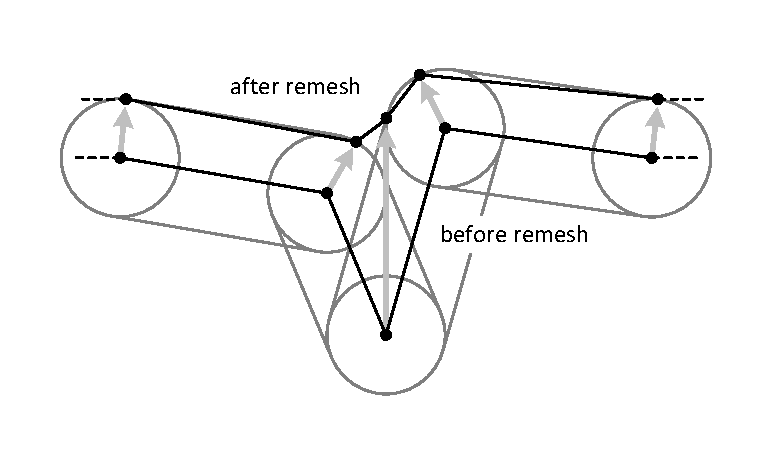
\includegraphics[width=\textwidth]{pics/pic_general_envelope_3_size.pdf}
    \caption{Иллюстрация затягивания впадины на 2D схеме.}\label{fig:pic_general_envelope_3_size}
  \end{minipage}
  \hfill
  \begin{minipage}[h]{0.44\textwidth}
    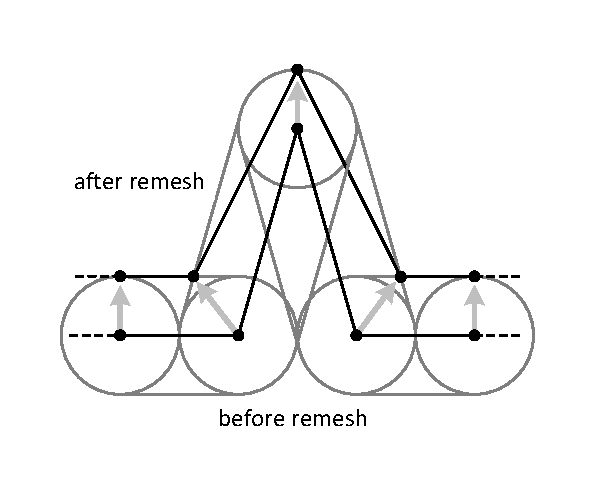
\includegraphics[width=\textwidth]{pics/pic_general_envelope_4_size.pdf}
    \caption{Иллюстрация сглаживания острого пика на 2D схеме.}\label{fig:pic_general_envelope_4_size}
  \end{minipage}
\end{figure}

\begin{figure}[h]
  \centering
  \begin{minipage}[h]{0.49\textwidth}
    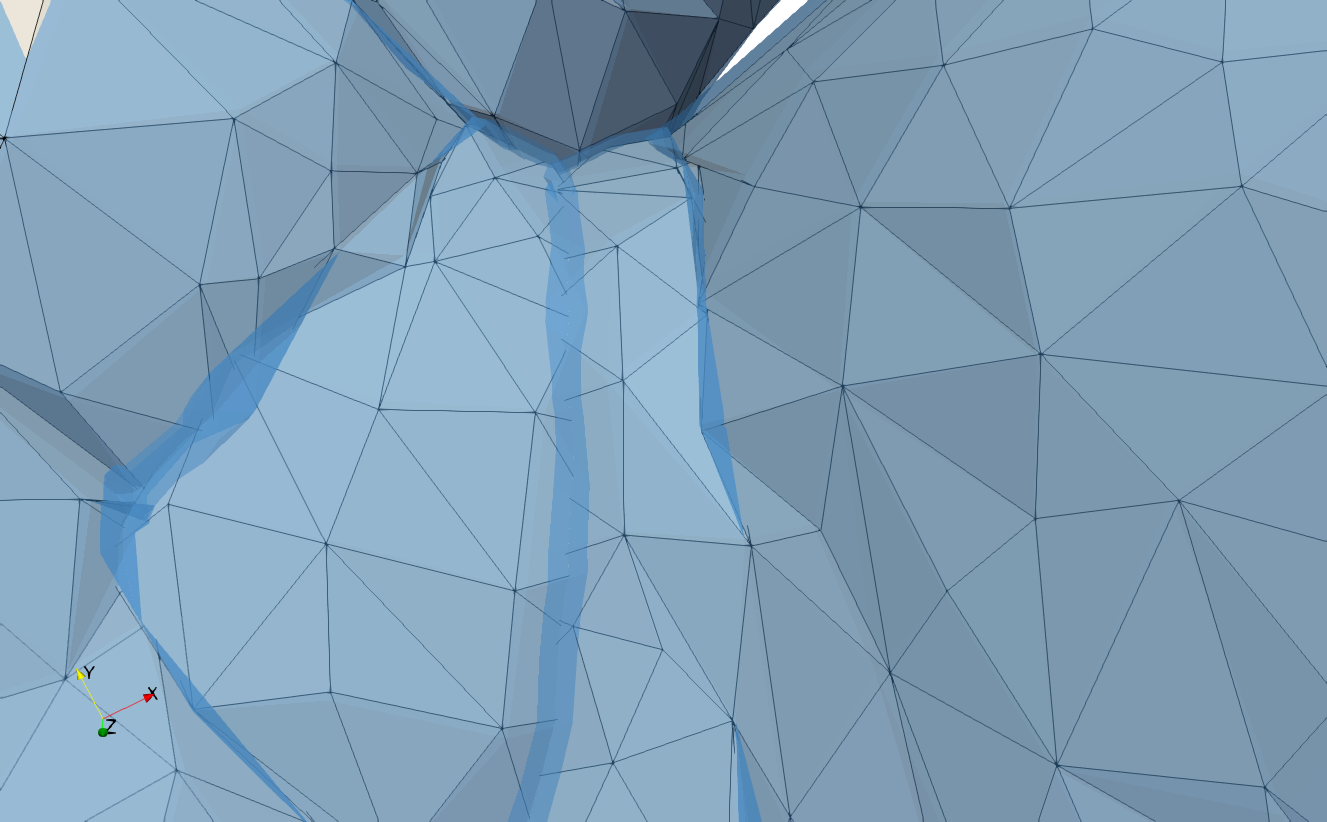
\includegraphics[width=\textwidth]{pics/pic_envelope_cave.png}
    \caption{Иллюстрация затягивания впадин для 3D поверхности.}\label{fig:pic_general_envelope_cave}
  \end{minipage}
  \hfill
  \begin{minipage}[h]{0.49\textwidth}
    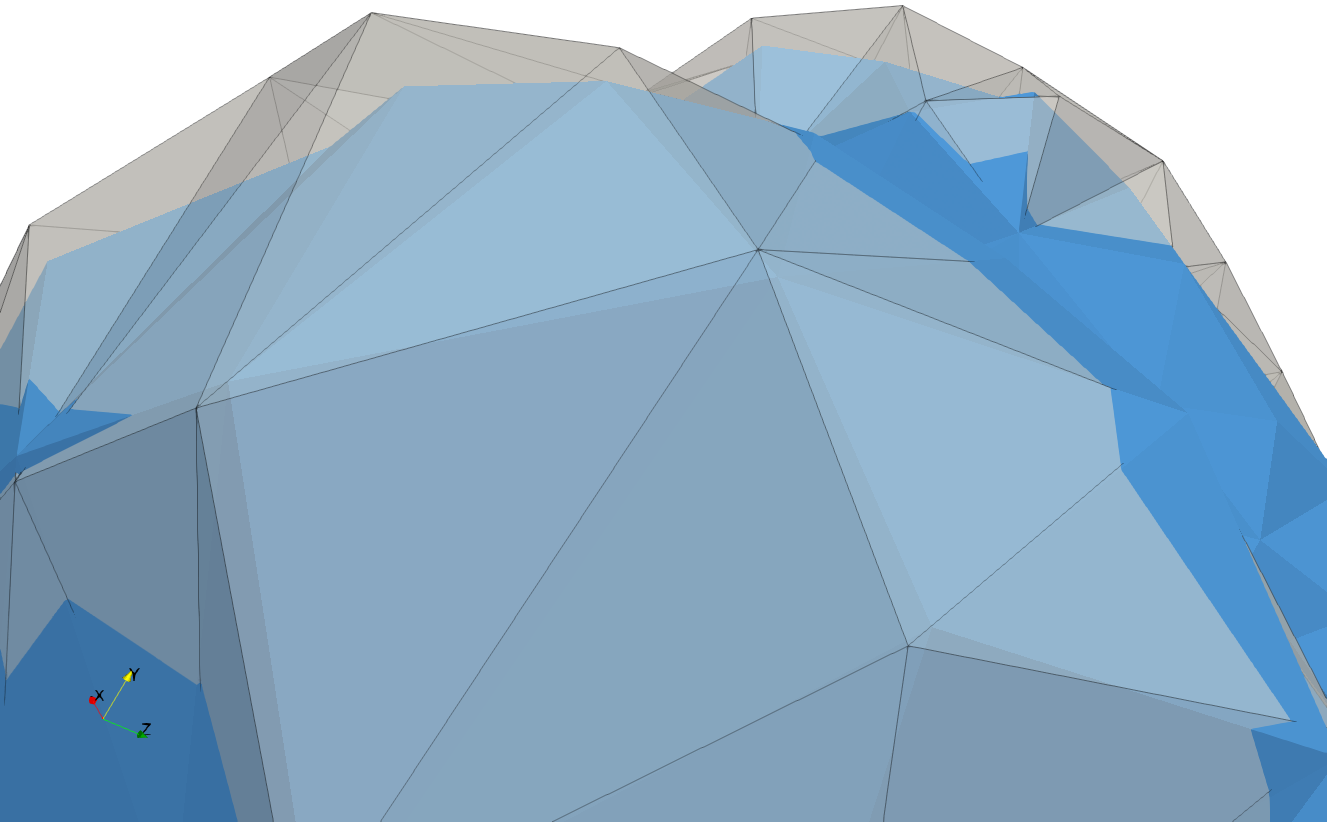
\includegraphics[width=\textwidth]{pics/pic_envelope_peak.png}
    \caption{Иллюстрация сглаживания острых пиков для 3D поверхности.}\label{fig:pic_envelope_peak}
  \end{minipage}
\end{figure}

Алгоритм определения новых положений узлов по общей огибающей семейства сфер является линейным по количеству узлов (считаем, что на пригодных к расчетам сетках количество инцидентных ячеек для одного узла ограничено разумным числом) и не содержит итерационных процедур.
Алгоритм обладает особенностью затягивать мелкие впадины и шумы на сетке.
Это происходит из-за того, что узел $\vec{N}$, находясь на дне впадины, имеет возможность смещаться по направлению выхода из этой впадины на расстояние, большее $R(\vec{N})$, что продемонстрировано на Fig.~\ref{fig:pic_general_envelope_3_size}.
Другой интересной особенностью является работа алгоритма на участках сетки с острыми выступами (Fig.~\ref{fig:pic_general_envelope_4_size}).
Из данного рисунка видно, что в процессе работы алгоритма острые пики имеют тенденцию к сглаживанию. 
Таким образом, новые положения узлов образуют более гладкую поверхность, чем она была до перестроения.

На Fig.~\ref{fig:pic_general_envelope_cave} продемонстрирован эффект затягивания впадин по сравнению с классическим методом призм (затягивание впадин на сетке отмечено синим цветом). На Fig.~\ref{fig:pic_envelope_peak} показан обратный эффект -- сглаживание острых пиков (по сравнению с тем же классическим методом призм).
